\documentclass{article}
\usepackage[utf8]{inputenc}
\usepackage[spanish]{babel}
\usepackage{amsthm}
\usepackage{amsmath}
\usepackage{amssymb}
\usepackage{graphicx}
\usepackage{wrapfig}
\usepackage[letterpaper, top=0.78in, bottom=0.78in, left=0.98in, right=0.98in]{geometry}
\usepackage{hyperref}
\usepackage{url}
\usepackage{soul}
\usepackage[document]{ragged2e}
\usepackage[table,xcdraw]{xcolor}
\usepackage{authblk}
\usepackage{enumitem}
\usepackage[font=footnotesize,labelfont=bf]{caption}

\providecommand{\keywords}[1]{\textbf{\textit{Index terms---}} #1}

\decimalpoint
\renewcommand{\baselinestretch}{1.5}
\newcolumntype{C}{>{\centering\arraybackslash}X}
\graphicspath{{../img/}}


\author{\normalsize Francisco Castorena Salazar}
\author{\normalsize Juan Pablo Echeagaray González}
\author{\normalsize Emily Rebeca Méndez Cruz}
\author{\normalsize José Eugenio Morales Ortiz}
\author{\normalsize Mario Javier Soriano Aguilera}
\affil{Ing. en Ciencias de Datos y Matemáticas, Tec de Monterrey}

\title{\Large \bf Descubriendo Periodicidad, Reconocimiento de Patrones y Modelos de Pronóstico de Aprendizaje Automático para El Niño-Oscilación del Sur mediante el Análisis Topológico de Datos}
\date{\normalsize 16 de junio del 2023}

\begin{document}
    \maketitle
    \begin{abstract}
        Este artículo explora la aplicación de técnicas de Análisis de Datos Topológicos (TDA, por sus siglas en inglés) en el contexto de los índices del fenómeno El Niño-Oscilación del Sur (ENSO) para identificar la periodicidad, descubrir anomalías y generar pronósticos. Se logró encontrar índices de periodicidad en todas las mediciones de ENSO a través del encaje de \textit{Takens} así como a través del algoritmo \textit{Mapper}. El modelo de pronóstico de ML desarrollado logró capturar la complejidad subyacente y la no linealidad del comportamiento de ENSO, lo que motiva el uso de TDA para obtener información más precisa.
    \end{abstract}

    \section{Introducción}

        El ENSO es un fenómeno climatológico que puede ser considerado en 3 partes principales: El niño (calentamiento de la superficie del oceano), La niña (Enfriamiento) o neutro donde hay una temperatura estable.

        Debido al error de los modelos sistemáticos, limitaciones de los modelos, y también a la dificultad que resultan las mediciones del ENSO debido a que es demasiado sensible a diversos cambios, fue que se opto por otro tipo de herramientas para poder análisis de los datos para predicciones y búsqueda de periodicidad.

        Este escrito se organiza de la siguiente manera en las secciones \ref{sec:theory} y \ref{sec:method} se describen los fundamentos teóricos y prácticos de las herramientas y técnicas a utilizar, así como una descripción detallada de cómo fueron aplicadas al caso de estudio. En la sección \ref{sec:results} se presentan los resultados obtenidos, los cuales son analizados en retrospectiva en la sección \ref{sec:discusion} y en la sección \ref{sec:conclusions} se presentan las conclusiones del estudio.

    \section{Marco Teórico} \label{sec:theory}

        \subsection{Takens Embedding}

            Este método esta basado en la técnica \emph{Time Delay Embedding}, la cual es una representación univariada de una serie de tiempo a partir de una nube de puntos \cite{gudhiembedding}.

            Se le conoce como \emph{Time Delay Embedding} a la manera de poder transformar una serie de tiempo a una matriz de tiempo la cual depende de pedazos de los datos \cite{timedelay}. Al transformar una secuencia larga de información a un set pequeño dependientes del tiempo, este se convierte en el centro del análisis en lugar de la predicción de variables en particular en una serie de tiempo.

            Dada una serie de tiempo discreto $(X_{0},X_{1},\dots)$ y una secuencia de muestras de tiempo separadas de manera uniforme $t_{0},t_{1},\dots$, se extrae un set $d$-dimensional de vectores de la forma $(X_{t_{i}},X_{t_{i}+\tau},\dots,X_{t_{i}+(d-1)\tau})$ para $i = 0,1,\dots$. Este set es el que se conoce como el \emph{Takens Embedding} de la serie de tiempo y la cual puede ser interpretada como una nube de puntos.

            La diferencia entre el tiempo $t_{i+1}$ y $t_{i}$ se conoce como \emph{stride} o paso, $\tau$ es conocido como el tiempo de retraso y \emph{d} se le atribuye a la dimensión del embedding.

        \subsection{Uniform Manifold Approximation and Projection}

            Uniform Manifold Approximation and Projection (UMAP) es una técnica de reducción de dimensiones que puede ser utilizado para visualización similar al t-SNE (t-Distributed Stochastic Neighbour Embedding), pero también es funcional con reducción general de dimensiones no lineales, dicho algoritmo funciona bajo 3 suposiciones \cite{umap}.

            \begin{itemize}[noitemsep]
                \item Los datos estan uniformemente distribuidos en un \emph{Riemannian manifold}.
                \item La métrica \emph{Riemannian} es localmente constante.
                \item El colector (manifold) esta localmente conectado.
            \end{itemize}

            Con estos supuestos se puede entonces dividir la construcción del algoritmo de UMAP en dos fases principales. La primera consiste en construir representación topológica difusa, después en la segunda fase consiste en la optimización de la reducción de dimensionalidad para acercarnos lo más posible a la representación topológica difusa la cual se mide mediante \emph{cross entropy}. Para más detalles se puede consultar la siguiente referencia \cite{umapworks}.

        \subsection{Spectral Embedding}

            \emph{Spectral Embedding} es un método no lineal de reducción de dimensionalidad, forma una matriz de afinidad dada por la función especifica y aplica descomposición espectral a la matriz laplaciana correspondiente, el resultado esta dado por el valor del eigenvector de cada punto de los datos \cite{spectral}.

            \emph{Spectral Embedding} es una aproximación al calculo de un encaje no lineal. La librería de Scikit-Learn utilizada implementa \emph{Laplacian Eigenmaps}, los cuales encuentran la representación de baja dimensión de los datos usando descomposición espectral de la matriz laplaciana, esta se puede considerar una aproximación discreta. La minimización de costo de la función asegura que los puntos cercanos unos a otros en el manifold sean mapeados cerca en el espacio de baja dimensión, preservando la distancia local \cite{spectralworks}.

        \subsection{Complejo Vietoris-Rips}

            El complejo de Vietoris-Rips es un complejo simplicial definido en un espacio métrico finito, este complejo suele ser usado como una aproximación del complejo de Čech debido a que el cálculo computacional de Vietoris-Rips es más rápido. \cite{vietoris}

            Dado un espacio métrico $(X,d_x)$ y $r > 0$ el complejo Vietoris-Rips asociado a r  $(VR_r(X))$, tiene a $X$ como su conjunto de elementos y sus complejos simpliciales son todos aquellos subconjuntos finitos no vacíos de X cuyo diámetro es estrictamente menor a $r$.\cite{Sunhyuk}

            La cantidad de complejos simpliciales de Vietoris-Rips puede ser muy grande, donde para una dimensión $k$ con $n$ puntos se pueden tener hasta $O(n^{k+1})$. Por lo cual, en la mayoría de los casos una reducción de dimensionalidad es necesaria.\cite{Yujie}

        \subsection{XGBoost}

            XGBoost es una librería que implementa algoritmos de aprendizaje automático bajo la técnica de Gradient Boosting, utilizando Gradient boosting Machines (GBM) para ser capaz de resolver muchos problemas predictivos de forma `rápida y precisa'.\cite{XGBoost}

            \subsubsection{Gradient Boosting}

                Este tipo de algoritmo es conocido por su capacidad de encontrar relaciones no lineales entre una variable objetivo y sus variables predictoras, por otra parte puede manejar valores faltantes, atípicos e incluso categóricos sin necesidad de tratamiento especial. Es una técnica de ensamble que combina múltiples modelos llamados débiles para poder crear un modelo fuerte, los débiles son arboles de decisión que se usan para ajustar el modelo y tener mejores predicciones.\cite{GradBoost}

    \section{Metodología} \label{sec:method}

        \subsection{Limpieza de bases de datos}

            Se realizará una limpieza de la base de datos proporcionada por ClimateAI así como de la base de datos general de la NOAA obtenida a través de la siguiente \href{https://www.cpc.ncep.noaa.gov/data/indices/sstoi.indices}{liga}. El formato de las bases de datos debe ser adecuado a uno tabular que sea sencillo de interpretar y de utilizar para los algoritmos de aprendizaje automático.

        \subsection{Análisis de Periodicidad}

            Dada una serie de tiempo obtenida de la limpieza de datos realizada, se realizará un corte de la serie de tiempo en ventanas arbitrarias; dichas ventanas serán procesadas con el algoritmo de \textit{Takens Embedding} para obtener una representación de la serie de tiempo en un espacio de dimensión superior. La selección de la dimensión de encaje y el retraso de tiempo serán determinados por el algoritmo de \textit{False Nearest Neighbors} y \textit{Mutual Information} respectivamente \cite{perea-time-series-tda}.

            La serie de tiempo transformada será sujeta a una reducción de dimensionalidad (UMAP o Spectral Embedding) a un espacio de 3 dimensiones; se estimará un diagrama de persistencia de Vietoris-Rips y la curva de números de Betti para la serie de tiempo procesada. Los resultados de estas operaciones serán visualizados para ser interpretados de forma manual y determinar si existe evidencia periodicidad en la serie de tiempo.

        \subsection{Reconocimiento de Patrones}

            El reconocimiento de patrones será acotado al análisis de los índices de anomalías \textit{ENSO} en la región 3.4; no se realizará ningún corte a esta serie de tiempo así como tampoco un tratamiento de valores atípicos, puesto que se trabajará bajo el supuesto de que el algoritmo \textit{Mapper} será lo suficientemente robusto para ignorar dichos valores.

            Para enriquecer el agrupamiento a realizar, se generarán 2 series de tiempo nuevas que contengan en sus observaciones el año y mes de ocurrencia de la medición respectivamente. Estas 3 características serán proyectadas al índice de anomalías Nino3.4; donde se generará una cubierta arbitraria en base la selección de cubos y traslape permitido.

            Dicha cubierta será agrupada con KMedias dada la distribución de campana que sigue esta variable; finalmente se generará una visualización del grafo compuesto para ser analizado de forma manual.

        \subsection{Modelado de Pronósticos}

            Se implementará un modelo de ML para pronosticar los índices de anomalías Nino3.4 en un horizonte de 40 meses. El modelo será informado por las propiedades topológicas de la serie de tiempo, en la figura \ref{fig:model_pipeline} se muestra el pipeline de modelado a implementar. Se generará una división de los datos en entrenamiento y prueba, dejando los últimos 40 meses para la prueba del modelo.

            La optimización de hiper-parámetros todavía no es soportada por la librería \textit{giotto}, por lo que se será pospuesta como trabajo futuro.
            \begin{figure}[!htbp]
                \centering
                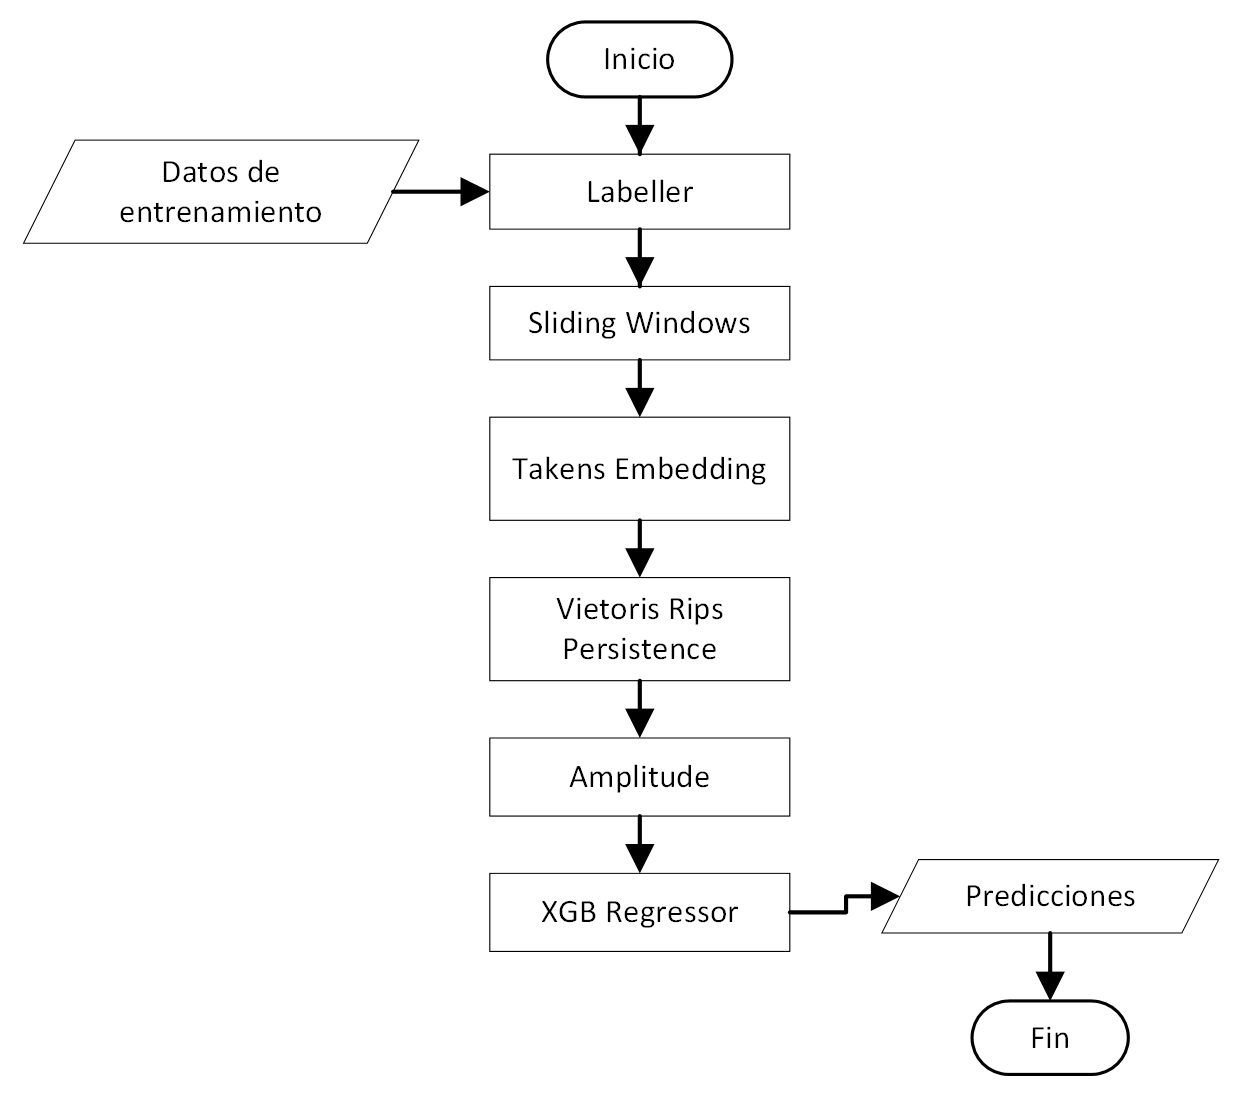
\includegraphics[width=0.5\textwidth]{model_pipeline.png}
                \caption{Pipeline de modelado}
                \label{fig:model_pipeline}
            \end{figure}

    \section{Experimentación y resultados}\label{sec:results}

        \subsection{Análisis de Periodicidad}

            En la figura \ref{fig:anom_nino_34_series} se despliega la serie de tiempo de índices de anomalías Nino 3.4 en una ventana de tiempo de 15 años comenzando en 1980.
            \begin{figure}[!htbp]
                \centering
                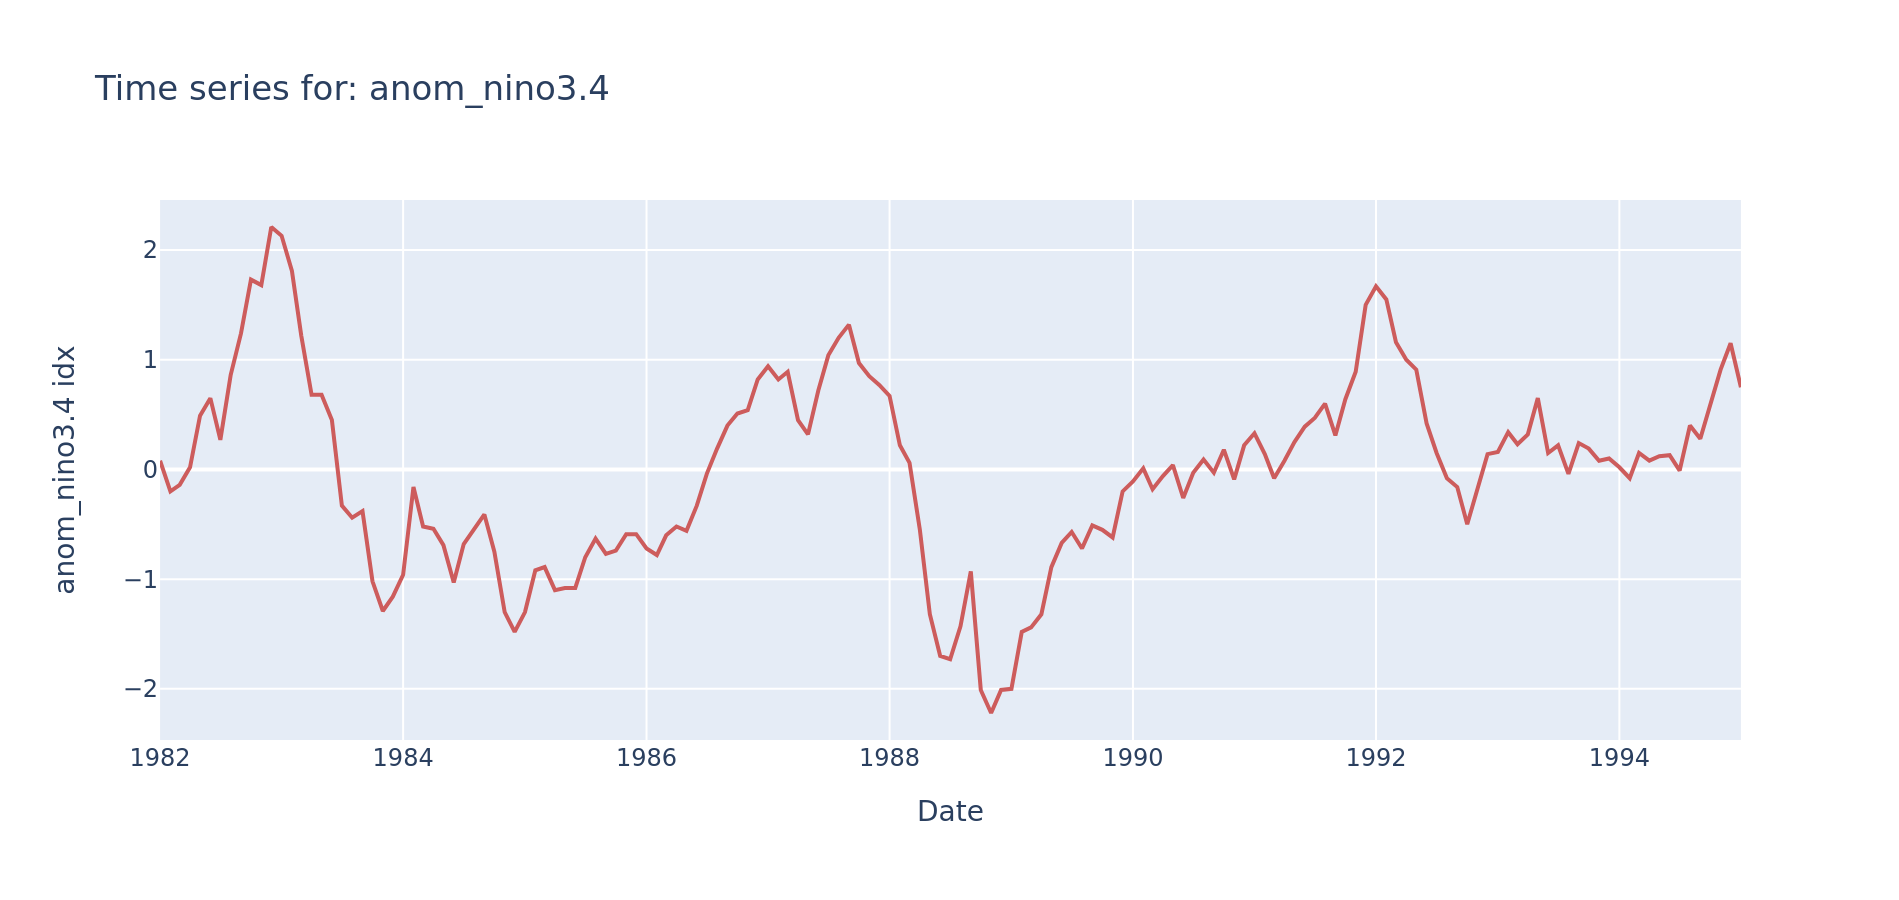
\includegraphics[scale=0.2]{anom_nino3.4_time_series.png}
                \caption{Serie de tiempo de índice de anomalías Nino 3.4, 1980 a 1995}
                \label{fig:anom_nino_34_series}
            \end{figure}

            La serie de tiempo fue procesada con el algoritmo de \textit{Takens Embedding}, la serie de tiempo fue proyectada a un espacio de 5 dimensiones con un retraso temporal de 2 observaciones. Dicha proyección fue a su vez reducida a un espacio de 3 dimensiones con el algoritmo de \textit{UMAP} con 4 componentes (figura \ref{fig:anom_nino34_proj}); se seleccionó este número de componentes bajo el supuesto de que la serie de tiempo contiene eventos del Niño, la Niña, eventos neutrales y una componente de ruido. Los diagramas de persistencia fueron calculados con el complejo de Vietoris-Rips (figura\ref{fig:anom_nino34_pers}), la complejidad computacional del algoritmo no representó un problema dada la reducción de dimensionalidad originada por el encaje.
            \begin{figure}[!htbp]
                \centering
                \begin{minipage}{0.45\textwidth}
                    \centering
                    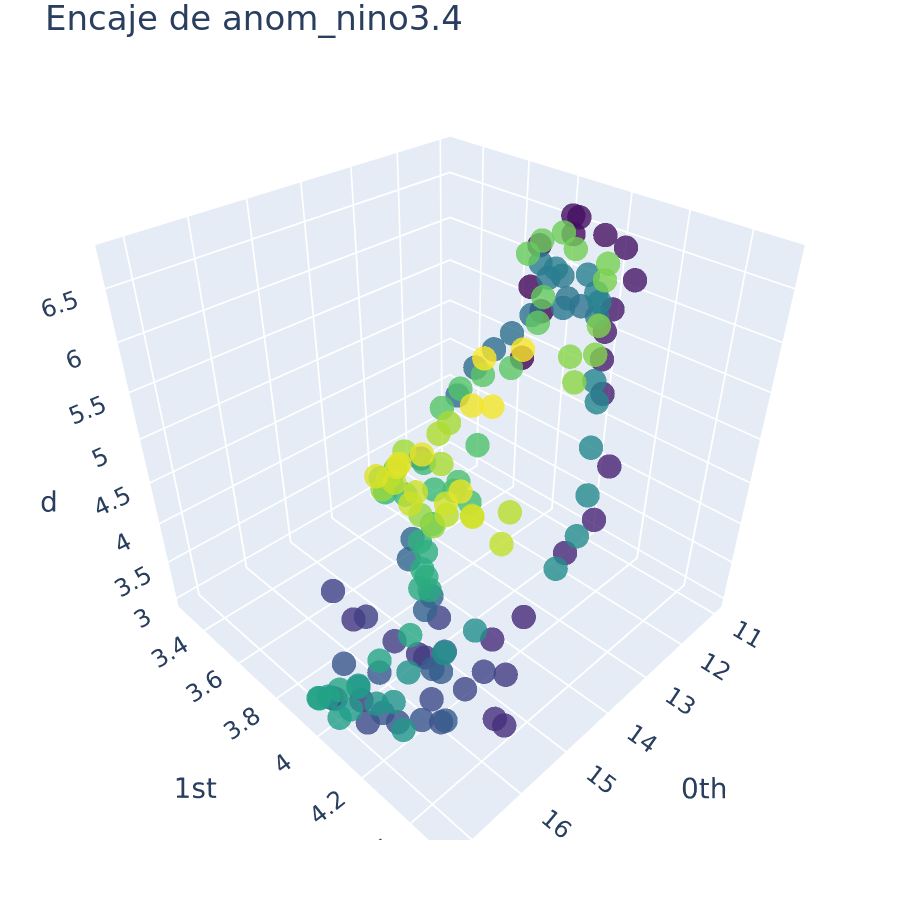
\includegraphics[scale=0.2]{anom_nino3.4_projection.png}
                    \caption{Proyección a 3 dimensiones con UMAP del encaje de Takens de Anom Nino3.4}
                    \label{fig:anom_nino34_proj}
                \end{minipage}
                \begin{minipage}{0.45\textwidth}
                    \centering
                    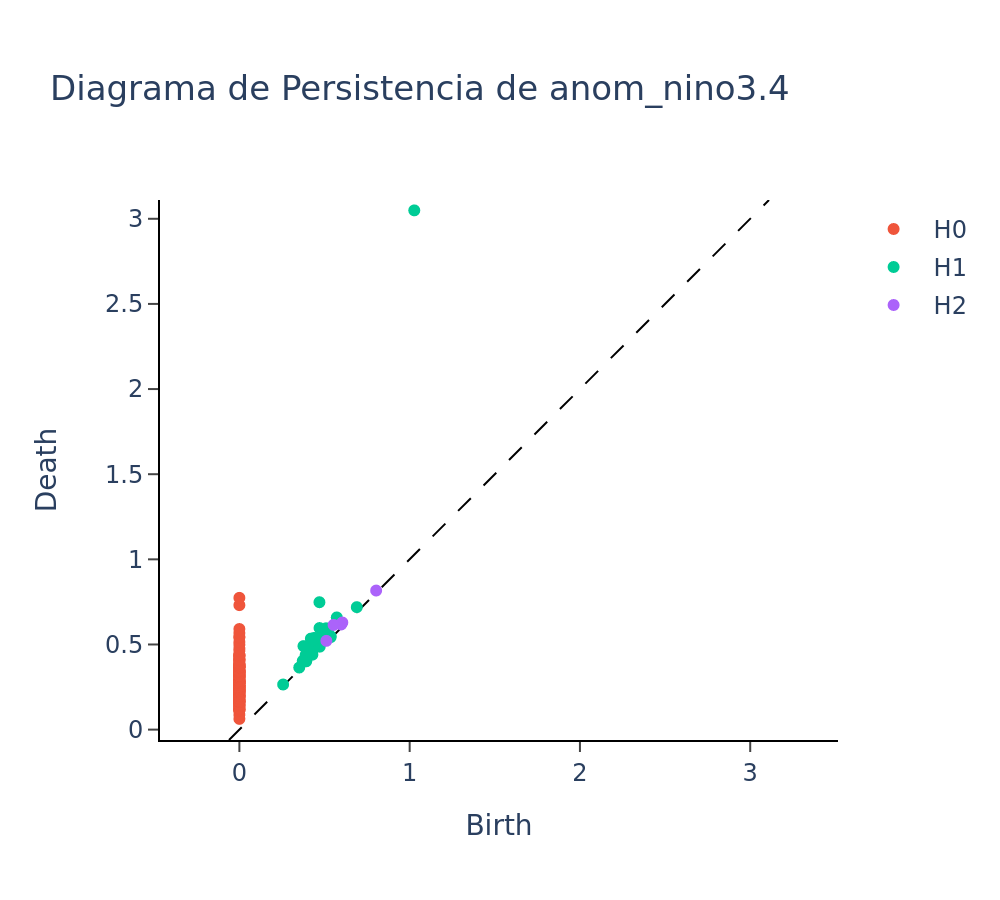
\includegraphics[scale=0.2]{anom_nino3.4_persistence.png}
                    \caption{Diagrama de Persistencia de Anom Nino3.4}
                    \label{fig:anom_nino34_pers}
                \end{minipage}
            \end{figure}

            En el diagrama de persistencia anterior se puede apreciar como se tiene un punto de $H_1$ que persiste por más tiempo que los demás puntos del tipo $H_1$ siendo este el hueco más grande que se tiene para la componente conexa generada, presentando evidencia suficiente como para afirmar que existe periodicidad en la serie de tiempo, la cual podemos comprobar de forma heurística al observar la forma de dona de la figura \ref{fig:anom_nino34_proj}. De forma general se encontraron índices de periodicidad en todas las series de tiempo proporcionadas; en la tabla \ref{tab:summary_embeddings} se presenta un sumario de los parámetros utilizados, y en la sección \ref{app:period} se presentan los diagramas de persistencia de cada serie de tiempo.
            \begin{table}[!htbp]
                \centering
                \scalebox{0.8}{
                \begin{tabular}{ |l|l|l|l|l| }
                \hline
                \textbf{Variable} & \textbf{Ventana de tiempo} & \textbf{Proyección} & \textbf{Dimensión de encaje} & \textbf{Retraso temporal} \\ \hline
                Nino 1.2 & 1980-2023 & Spectral Embedding & 8 & 3 \\ \hline
                Anom Nino1.2 & 2000-2020 & UMAP & 6 & 2 \\ \hline
                Nino3 & 1992-2005 & UMAP & 6 & 1 \\ \hline
                Anom Nino3 & 1980-1995 & UMAP & 7 & 3 \\ \hline
                Nino3.4 & 1982-2006 & UMAP & 7 & 4 \\ \hline
                Anom Nino3.4 & 1980-1995 & UMAP & 5 & 2 \\ \hline
                Nino4 & 1980-1997 & UMAP & 7 & 3 \\ \hline
                Anom Nino4 & 1980-2023 & UMAP & 8 & 10 \\ \hline
                \end{tabular}}
                \caption{Resumen de encajes de Takens y proyecciones}
                \label{tab:summary_embeddings}
            \end{table}

        \subsection{Reconocimiento de patrones}

            En la figura \ref{fig:mapper_graph} se despliega el grafo creado por el algoritmo \textit{Mapper} al tratar de agrupar las observaciones de anomalías Nino 3.4. Se destaca que el grafo generado tiene forma de cuerda, donde no quedó ningún nodo desconectado de la red, y con cada nodo teniendo una distribución de valores distinta, representada por el índice de anomalías.
            \begin{figure}[!htbp]
                \centering
                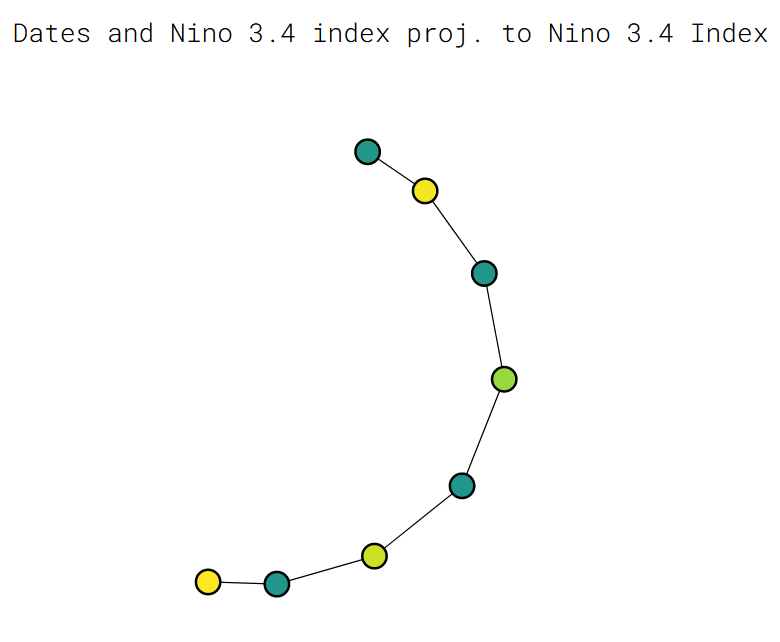
\includegraphics[scale=0.5]{mapper_full_anom_nino34_chord.png}
                \caption{Grafo de línea generado por Mapper en Anom Nino3.4}
                \label{fig:mapper_graph}
            \end{figure}

            La secuencia de nodos \textit{calientes} a \textit{fríos} que sucede en todo el grafo lleva a pensar que \textit{Mapper} tal vez esté capturando la naturaleza periódica del fenómeno. En la figura \ref{fig:mapper_periodicity} se despliegan las series de tiempo de 4 nodos (caliente a frío).

            Notamos que al agrupar los nodos en tuplas (caliente, frío) los meses de la serie de tiempo siempre son respetados, garantizando una continuidad entre todas las observaciones; aunado a esto, se logra llegar a una separación de observaciones mayoritariamente frías de las calientes; el equipo conjetura que estas agrupaciones naturales en conjunto con la continuidad de las observaciones son evidencia considerable de que el algoritmo \textit{Mapper} captura de forma adecuada la naturaleza periódica del fenómeno.
            \begin{figure}[!htbp]
                \centering
                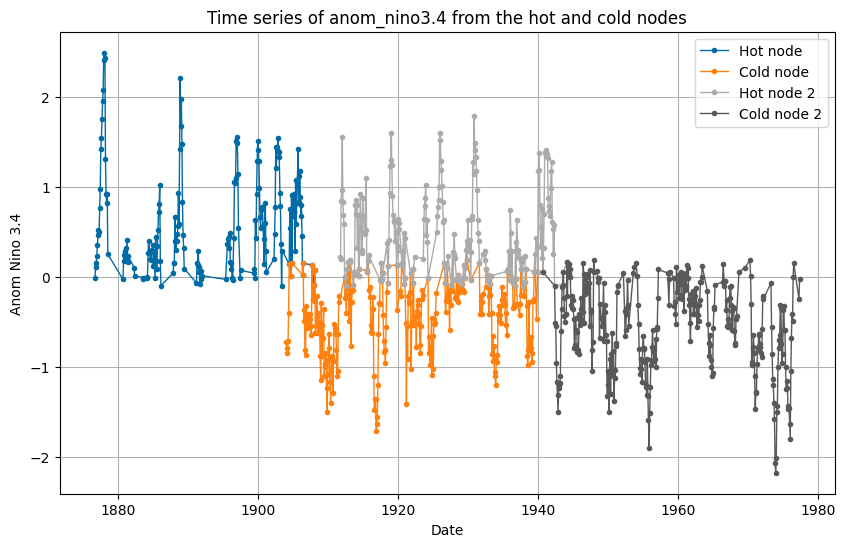
\includegraphics[scale=0.5]{mapper_periodicity.png}
                \caption{Muestra de clústers definidos por Mapper en Anom Nino3.4}
                \label{fig:mapper_periodicity}
            \end{figure}

        \subsection{Modelo de pronóstico}

            Una vez hecha la separación en datos de entrenamiento y prueba, se entrenó un regresor XGB sobre las características topológicas de la serie de tiempo Anom Nino 3.4; en la figura \ref{fig:anom_nino34_forecast} se despliega una muestra de predicciones que va desde 1880 a 1940. Destacamos que la serie de tiempo no presenta un sobre-ajuste a los datos, pero sí logra capturar la forma misma de la serie; indicando que las características extraídas del TDA fueron lo suficientemente informativas como para que el modelo de pronóstico pudiera aprender la forma de la serie de tiempo.
            \begin{figure}[!htbp]
                \centering
                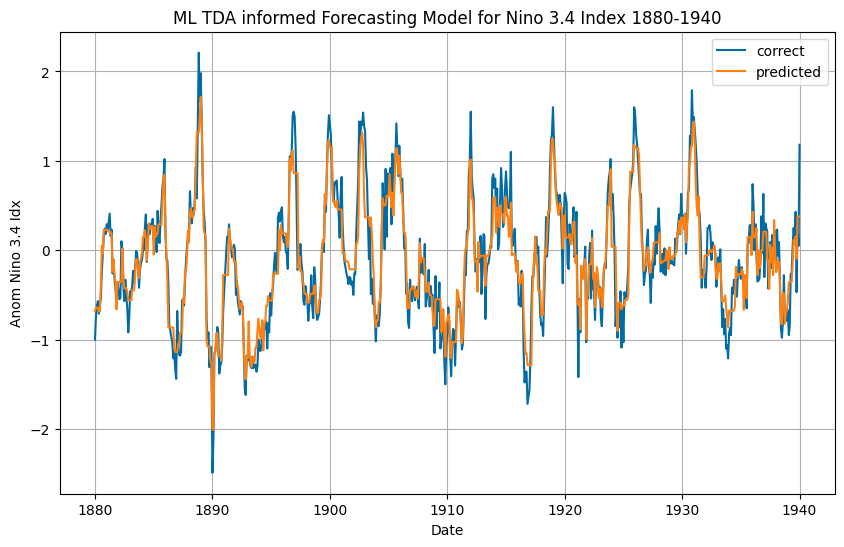
\includegraphics[scale=0.5]{forecasting_ml_xgb.png}
                \caption{Pronóstico de Anom Nino3.4}
                \label{fig:anom_nino34_forecast}
            \end{figure}

            En la figura \ref{fig:anom_nino34_forecast_test} se presentan las 40 predicciones qe realizó el modelo en los datos de prueba. En este caso aislado notamos que el modelo logró capturar la tendencia de la serie de tiempo con éxito, más no así los valores exactos de la misma. El \textit{MAPE} de este modelo fue de $1.58\%$.
            \begin{figure}[!htbp]
                \centering
                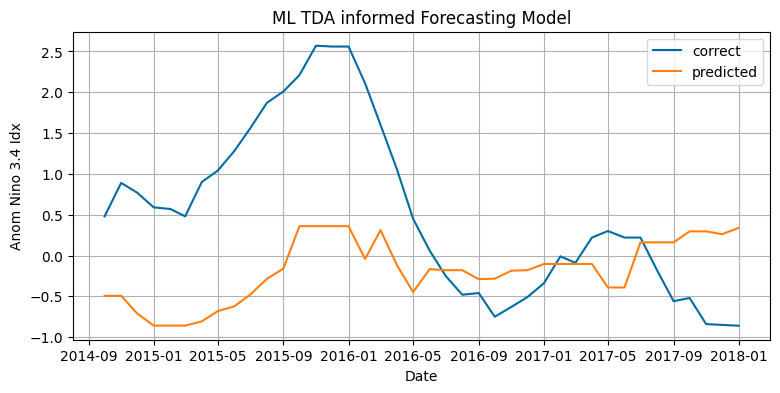
\includegraphics[scale=0.5]{forecasting_ml_xgb_test.png}
                \caption{Pronóstico en datos de prueba}
                \label{fig:anom_nino34_forecast_test}
            \end{figure}

    \section{Discusión de resultados}\label{sec:discusion}

        \subsection{Generalización de análisis de periodicidad}

            Actualmente el análisis implementado para la búsqueda de periodicidad para todas las variables a excepción de Anom Nino3.4 quedaron confinadas a observaciones a partir de 1980; la inclusión de datos históricos que cubran desde 1880 (como lo es con Anom Nino3.4) enriquecería el estudio realizado, así como también permitiría una mejor generalización de los resultados obtenidos.

        \subsection{Funciones de proyección para Mapper}

            El agrupamiento con Mapper realizado también se vio mermado por el grado de información disponible para las mediciones del índice de anomalías de Nino 3.4; se considera que al disponer de un mayor número de observaciones para las demás variables, se podría hacer uso de funciones de proyección y agrupamiento más complejas en el proceso de generación de cubos y clusters, incrementando aún más el grado de análisis de las relaciones de interdependencia entre las variables.

        \subsection{Optimización de hiper-parámetros de modelo de pronóstico}

            El pipeline de características topológicas de la serie de tiempo que hemos utilizado todavía no soporta la optimización de hiper-parámetros en un conjunto de datos de validación; sin embargo consideramos que este es un límite suave que está en vías de ser solventado en la próxima iteración de la librería \textit{Giotto-TDA}.

    \section{Conclusiones}\label{sec:conclusions}

        El análisis de periodicidad y pronóstico de los índices de El Niño sigue siendo uno de los principales desafíos en los cuáles el Análisis Topológico de Datos puede ofrecer una perspectiva de estudio completamente distinta

        En este trabajo se ha logrado demostrar y cuantificar la presencia de periodicidad en las series de tiempo de El Niño a través de técnicas de TDA; dicha periodicidad fue también descubierta al hacer uso de métodos de clusterización con cualidades topológicas, las mismas funciones que permitieron el descubrimiento de periodicidad facilitaron la creación de un modelo de pronóstico que logró capturar la forma de la serie de tiempo.

    \clearpage
    \bibliographystyle{IEEEtran}
    \bibliography{references.bib}

    \clearpage
    \appendix
    \section{Código}

        Consultar código en la siguiente \href{https://github.com/JuanEcheagaray75/elnino_tda}{liga}.

\end{document}
